\chapter{Analisi dei requisiti}
\label{chap:analisi-requisiti}

\section{Tipologie di utenti}

All'interno del sistema vengono individuati tre principali attori coinvolti nell'interazione con le funzionalità sviluppate:

\begin{itemize}
    \item \textbf{Utente:} dipendente dell'azienda utilizzatrice del software, rappresenta il principale utilizzatore del gestionale. 
    Interagisce con il sistema per consultare informazioni, ricevere segnalazioni relative a eventuali criticità e richiedere spiegazioni sulle decisioni prodotte 
    dai diversi moduli applicativi.

    \item \textbf{Utente amministratore:} dipendente dell'azienda con privilegi avanzati rispetto all'utente base. Possiede tutte le funzionalità disponibili per quest'ultimo 
    e può modificare configurazioni e impostazioni del sistema non accessibili agli utenti standard.

    \item \textbf{Sistema ERP:} componente principale del gestionale responsabile dell'elaborazione delle informazioni operative. Si occupa di monitorare le 
    condizioni definite nelle regole degli alert configurate dagli utenti e di generare le relative segnalazioni in caso di violazione dei criteri stabiliti.

    \item \textbf{Modulo XAI:} componente software basato su chatbot che consente all'utente di interrogare il sistema e ottenere informazioni o spiegazioni 
    relative alle decisioni prese dal gestionale. Il modulo può utilizzare meccanismi di \textit{function calling} per recuperare dati dal database o eseguire 
    operazioni specifiche, come la creazione di nuovi record relativi ad acquisti o vendite, previa conferma esplicita dell'utente.
\end{itemize}


\section{Casi d'uso}
I casi d'uso rappresentano una descrizione delle principali interazioni tra gli attori del sistema e le funzionalità offerte dall'applicazione. Essi permettono di 
definire i comportamenti attesi del sistema dal punto di vista degli utenti, descrivendo gli obiettivi che ciascun attore può raggiungere attraverso l'utilizzo delle 
funzionalità disponibili.
\newline
La rappresentazione dei casi d'uso consente quindi di fornire una visione ad alto livello dei requisiti funzionali del sistema, evidenziando le modalità con cui gli utenti 
interagiscono con il gestionale e con le nuove funzionalità introdotte.
\newline
Ogni caso d'uso è accompagnato dal relativo diagramma \gls{uml}, che permette di rappresentare graficamente gli attori coinvolti e le interazioni con il sistema, rendendo più 
chiara e immediata la comprensione delle funzionalità descritte.


\subsection{Struttura dei casi d'uso}

\begin{center}
    \rowcolors{2}{lightblue}{white}
        \begin{tabularx}{\textwidth}{|l|X|}
            \hline
            \rowcolor{gold}
            \textbf{Campo}  & \textbf{Descrizione} \\
            \hline
            \textbf{Attori} & Indica gli utenti o i componenti del sistema coinvolti nell'esecuzione del caso d'uso e che interagiscono direttamente con la funzionalità descritta.\\
            \hline
            \textbf{Precondizioni} & Definisce le condizioni che devono essere soddisfatte prima dell'avvio del caso d'uso affinché questo possa essere eseguito correttamente.\\
            \hline
            \textbf{Postcondizioni} & Descrive lo stato del sistema al termine dell'esecuzione del caso d'uso e gli eventuali risultati prodotti dall'interazione.\\
            \hline
            \textbf{Scenario principale} & Rappresenta il flusso di esecuzione standard del caso d'uso, descrivendo le operazioni effettuate dagli attori e le risposte 
            fornite dal sistema.\\
            \hline
            \textbf{Scenari alternativi} & Descrive eventuali variazioni rispetto al flusso principale, dovute a condizioni particolari o situazioni differenti che possono 
            verificarsi durante l'esecuzione.\\
            \hline
            \textbf{Inclusioni} & Indica altri casi d'uso che vengono richiamati obbligatoriamente dal caso d'uso corrente e che rappresentano funzionalità comuni riutilizzate.\\
            \hline
            \textbf{Estensioni} & Indica eventuali comportamenti aggiuntivi o opzionali che possono estendere il caso d'uso principale al verificarsi di specifiche condizioni.\\
            \hline
        \end{tabularx}
\end{center}

% \begin{figure}[H]
%     \vspace{2em}
%     \centering
%     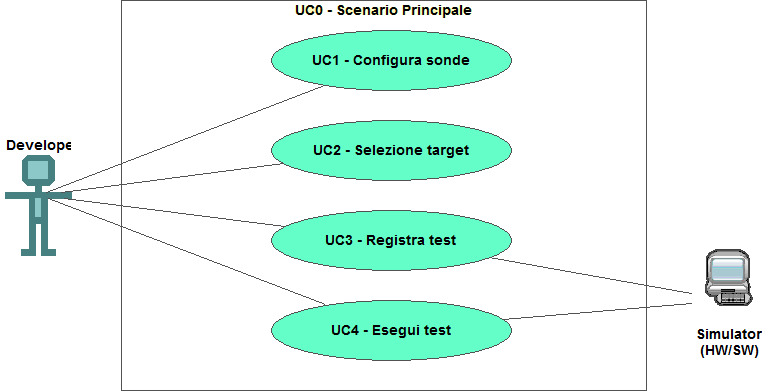
\includegraphics[alt={Testo alternativo dell'immagine}, width=0.75\columnwidth]{img/usecase/scenario-principale.jpeg}
%     \caption{Use Case 0: Scenario principale}
%     \label{fig:scenario_principale}
% \end{figure}
\section{Elenco casi d'uso}

\subsection{UC1: Configurazione del modulo XAI}
\label{uc:uc1}
    \begin{itemize}
        \item \textbf{Attori:} Utente amministratore.
        \item \textbf{Precondizioni:} 
            \begin{enumerate}
                \item l'utente è autenticato; 
                \item l'utente possiede i permessi di amministratore.
            \end{enumerate}
        \item \textbf{Postcondizioni:} il modulo XAI risulta configurato secondo le impostazioni definite dall'amministratore e disponibile per gli utenti autorizzati.
        \item \textbf{Scenario principale:}
            \begin{enumerate}
                \item L'amministratore entra nella pagina contenente le impostazioni del modulo XAI.
                \item L'amministratore seleziona il modello LLM che vuole far utilizzare agli utenti (\hyperref[uc:uc1.1]{UC1.1}).
                \item L'amministratore permette a tutte le categorie di utenti di utilizzare il modulo XAI (\hyperref[uc:uc1.2]{UC1.2}).
                \item L'amministratore seleziona i \textit{tool} che vuole far utilizzare al chatbot (\hyperref[uc:uc1.3]{UC1.3}). 
            \end{enumerate}
        \item \textbf{Inclusioni:}
            \begin{enumerate}
                \item \hyperref[uc:uc1.1]{UC1.1: Selezione del modello LLM per il modulo XAI}
                \item \hyperref[uc:uc1.2]{UC1.2: Configurazione degli utenti abilitati al modulo XAI}
                \item \hyperref[uc:uc1.3]{UC1.3: Configurazione dei tool disponibili per il modulo XAI}
            \end{enumerate}
    \end{itemize}
    

\subsubsection{UC1.1: Selezione del modello LLM per il modulo XAI}
\label{uc:uc1.1}
    \begin{itemize}
        \item \textbf{Attori:} Utente amministratore.
        \item \textbf{Precondizioni:} 
            \begin{enumerate}
                \item L'amministratore si trova all'interno della pagina di impostazioni del modulo XAI.
            \end{enumerate}
        \item \textbf{Postcondizioni:} Il modulo XAI è configurato per utilizzare il modello LLM selezionato dall'amministratore.
        \item \textbf{Scenario principale:}
            \begin{enumerate}
                \item L'amministratore seleziona il provider da utilizzare.
                \item L'amministratore seleziona il modello specifico da utilizzare.
            \end{enumerate}
    \end{itemize}
    

\subsubsection{UC1.2: Configurazione degli utenti abilitati al modulo XAI}
\label{uc:uc1.2}
    \begin{itemize}
        \item \textbf{Attori:} Utente amministratore.
        \item \textbf{Precondizioni:} 
            \begin{enumerate}
                \item L'amministratore si trova all'interno della pagina di impostazioni del modulo XAI.
            \end{enumerate}
        \item \textbf{Postcondizioni:} Il modulo XAI è configurato per poter essere utilizzato dagli utenti utilizzatori del sistema.
        \item \textbf{Scenario principale:}
            \begin{enumerate}
                \item L'amministratore seleziona i gruppi di utenti a cui concedere l'accesso al chatbot.
            \end{enumerate}
    \end{itemize}
    

\subsubsection{UC1.3: Configurazione dei tool disponibili per il modulo XAI}
    \label{uc:uc1.3}
    \begin{itemize}
        \item \textbf{Attori:} Utente amministratore.
        \item \textbf{Precondizioni:} 
            \begin{enumerate}
                \item L'amministratore si trova all'interno della pagina di impostazioni del modulo XAI.
            \end{enumerate}
        \item \textbf{Postcondizioni:} Il modulo XAI è configurato per poter utilizzare i tool selezionati dall'amministratore.
        \item \textbf{Scenario principale:}
            \begin{enumerate}
                \item L'amministratore seleziona i tool che desidera rendere visibili al chatbot.
            \end{enumerate}
    \end{itemize}


\subsection{UC2: Richiesta di spiegazioni al modulo XAI su una decisione del sistema}
\label{uc:uc2}
    \begin{itemize}
        \item \textbf{Attori:} Utente, Modulo XAI.
        \item \textbf{Precondizioni:} 
            \begin{enumerate}
                \item L'utente è autenticato; 
                \item L'utente possiede i permessi per poter utilizzare il chatbot;
                \item Il modulo XAI ha i tool per fare richieste abilitati.
            \end{enumerate}
        \item \textbf{Postcondizioni:} L'utente riceve una spiegazione dal modulo XAI riguardo le decisioni prese dal gestionale.
        \item \textbf{Scenario principale:}
            \begin{enumerate}
                \item L'utente attiva la sidebar relativa al modulo XAI.
                \item L'utente accede ad una conversazione con il modulo XAI (\hyperref[uc:uc2.1]{UC2.1}).
                \item L'utente scrive una richiesta di spiegazioni nella chat. 
                \item Il chatbot effettua una chiamata a tool per poter ricevere i dati (\hyperref[uc:uc2.2]{UC2.2}).
                \item Il chatbot elabora i dati e li dà in output all'utente in linguaggio naturale.
            \end{enumerate}
        \item \textbf{Scenari alternativi:}
            \begin{enumerate}
                \item Il modello LLM non è raggiungibile e non è possibile generare la risposta (\hyperref[uc:uc2.3]{UC2.3}).
                \item Le informazioni recuperate superano il limite massimo di token elaborabili dal modello (\hyperref[uc:uc2.4]{UC2.4}).
                \item L'utente non dispone dei permessi necessari per visualizzare le informazioni richieste (\hyperref[uc:uc2.5]{UC2.5}).
            \end{enumerate}
        \item \textbf{Inclusioni:}
            \begin{enumerate}
                \item \hyperref[uc:uc2.1]{UC2.1: Gestione della conversazione con il modulo XAI}
                \item \hyperref[uc:uc2.2]{UC2.2: Chiamata a tool per spiegazioni del modulo XAI}
            \end{enumerate}
        \item \textbf{Estensioni:}
            \begin{enumerate}
                \item \hyperref[uc:uc2.3]{UC2.3: Modello LLM non raggiungibile}
                \item \hyperref[uc:uc2.4]{UC2.4: Limite token di risposta superato}
                \item \hyperref[uc:uc2.5]{UC2.5: Permessi non sufficienti per effettuare la richiesta}
            \end{enumerate}
    \end{itemize}

\subsubsection{UC2.1: Gestione della conversazione con il modulo XAI}
\label{uc:uc2.1}
    \begin{itemize}
        \item \textbf{Attori:} Utente.
        \item \textbf{Precondizioni:}
            \begin{enumerate}
                \item L'utente è autenticato;
                \item L'utente possiede i permessi per utilizzare il modulo XAI.
            \end{enumerate}
        \item \textbf{Postcondizioni:} L'utente accede ad una conversazione già iniziata con il modulo XAI.
        \item \textbf{Scenario principale:}
            \begin{enumerate}
                \item L'utente apre la sidebar relativa al modulo XAI.
                \item L'utente seleziona una conversazione esistente.
                \item Il sistema carica il contesto della conversazione selezionata.
            \end{enumerate}
        \item \textbf{Scenario alternativo:}
            \begin{enumerate}
                \item L'utente crea una nuova conversazione senza uno storico precedente.
            \end{enumerate}
    \end{itemize}


\subsubsection{UC2.2: Chiamata a tool per spiegazioni del modulo XAI}
    \label{uc:uc2.2}
    \begin{itemize}
        \item \textbf{Attori:} Modulo XAI.
        \item \textbf{Precondizioni:} 
            \begin{enumerate}
                \item L'utente ha inviato una richiesta di spiegazioni al chatbot.
            \end{enumerate}
        \item \textbf{Postcondizioni:} Il modulo XAI possiede i dati per rispondere all'utente.
        \item \textbf{Scenario principale:}
            \begin{enumerate}
                \item Il modulo XAI, in base alla richiesta, sceglie il tool di spiegazioni da chiamare per compiere il suo obiettivo.
                \item Il tool effettua le query a database necessarie per poter ricavare i dati da dare in output all'utente.
                \item Il tool formatta i dati ricevuti in un formato leggibile dall'LLM.
            \end{enumerate}
    \end{itemize}

\subsubsection{UC2.3: Modello LLM non raggiungibile}
    \label{uc:uc2.3}
    \begin{itemize}
        \item \textbf{Attori:} Utente.
        \item \textbf{Precondizioni:} 
            \begin{enumerate}
                \item L'utente ha inviato una richiesta di spiegazioni al modulo XAI.
            \end{enumerate}
        \item \textbf{Postcondizioni:} L'applicazione ritorna un errore.
        \item \textbf{Scenario principale:}
            \begin{enumerate}
                \item Il modulo XAI non è raggiungibile dall'applicazione.
            \end{enumerate}
    \end{itemize}


\subsubsection{UC2.4: Limite token di risposta superato}
    \label{uc:uc2.4}
    \begin{itemize}
        \item \textbf{Attori:} Utente.
        \item \textbf{Precondizioni:} 
            \begin{enumerate}
                \item L'utente ha inviato una richiesta di spiegazioni al modulo XAI.
            \end{enumerate}
        \item \textbf{Postcondizioni:} L'applicazione ritorna un errore.
        \item \textbf{Scenario principale:}
            \begin{enumerate}
                \item Il sistema rileva che la quantità di dati da fornire al modello supera il limite massimo di token consentito.
            \end{enumerate}
    \end{itemize}


\subsubsection{UC2.5: Permessi non sufficienti per effettuare la richiesta}
    \label{uc:uc2.5}
    \begin{itemize}
        \item \textbf{Attori:} Utente.
        \item \textbf{Precondizioni:}
            \begin{enumerate}
                \item L'utente ha inviato una richiesta di spiegazioni al modulo XAI.
            \end{enumerate}
        \item \textbf{Postcondizioni:} Il modulo XAI comunica all'utente che non possiede i permessi per poter ricevere la spiegazione.
        \item \textbf{Scenario principale:}
            \begin{enumerate}
                \item Il modulo XAI rileva che i tool che utilizza per la risposta fanno uso di modelli a cui l'utente non ha accesso.
            \end{enumerate}
    \end{itemize}

\subsection{UC3: Richiesta creazione nuovi record}
\label{uc:uc3}
    \begin{itemize}
        \item \textbf{Attori:} Utente, Modulo XAI.
        \item \textbf{Precondizioni:} 
            \begin{enumerate}
                \item L'utente è autenticato; 
                \item L'utente possiede i permessi per poter utilizzare il chatbot;
                \item Il modulo XAI ha i tool per poter creare nuovi record abilitati.
            \end{enumerate}
        \item \textbf{Postcondizioni:} L'utente crea un nuovo record relativo ai dati forniti al chatbot.
        \item \textbf{Scenario principale:}
            \begin{enumerate}
                \item L'utente attiva la sidebar relativa al modulo XAI.
                \item L'utente accede ad una conversazione con il modulo XAI (\hyperref[uc:uc2.1]{UC2.1}).
                \item L'utente scrive una richiesta di creazione record nella chat.
                \item L'utente fornisce i dati necessari alla creazione del record.
                \item Il chatbot effettua una chiamata a tool per poter creare il form (\hyperref[uc:uc3.1]{UC3.1}).
                \item Il chatbot richiede la conferma dei dati previa creazione del record.
            \end{enumerate}
        \item \textbf{Scenari alternativi:}
            \begin{enumerate}
                \item Il modello LLM non è raggiungibile e non è possibile generare la risposta (\hyperref[uc:uc2.3]{UC2.3}).
                \item Le informazioni recuperate superano il limite massimo di token elaborabili dal modello (\hyperref[uc:uc2.4]{UC2.4}).
                \item L'utente non dispone dei permessi necessari per poter creare il record (\hyperref[uc:uc2.5]{UC2.5}).
                \item I dati forniti dall'utente sono incorretti per la creazione del record (\hyperref[uc:uc3.2]{UC3.2}).
            \end{enumerate}
        \item \textbf{Inclusioni:}
            \begin{enumerate}
                \item \hyperref[uc:uc2.1]{UC2.1: Gestione della conversazione con il modulo XAI}
                \item \hyperref[uc:uc3.1]{UC3.1: Chiamata a tool del modulo XAI}
            \end{enumerate}
        \item \textbf{Estensioni:}
            \begin{enumerate}
                \item \hyperref[uc:uc2.3]{UC2.3: Modello LLM non raggiungibile}
                \item \hyperref[uc:uc2.4]{UC2.4: Limite token di risposta superato}
                \item \hyperref[uc:uc2.5]{UC2.5: Permessi non sufficienti per effettuare la richiesta}
                \item \hyperref[uc:uc3.2]{UC3.2: Dati forniti incorretti per la creazione del record}
            \end{enumerate}
    \end{itemize}

\subsubsection{UC3.1: Chiamata al tool per creazione record del modulo XAI}
    \label{uc:uc3.1}
    \begin{itemize}
        \item \textbf{Attori:} Utente.
        \item \textbf{Precondizioni:}
            \begin{enumerate}
                \item L'utente ha inviato una richiesta di creazione record al modulo XAI.
            \end{enumerate}
        \item \textbf{Postcondizioni:} Il modulo XAI fornisce all'utente un form compilato con tutti i dati forniti.
        \item \textbf{Scenario principale:}
            \begin{enumerate}
                \item Il modulo XAI richiama i tool per la creazione di un nuovo record.
                \item Il modulo XAI controlla che i campi corrispondano alla richiesta dell'utente.
            \end{enumerate}
        \item \textbf{Scenario alternativo:}
            \begin{enumerate}
                \item Il modulo XAI rileva che i campi non corrispondono alle richieste dell'utente.
            \end{enumerate}
        \item \textbf{Estensioni:}
            \begin{enumerate}
                \item \hyperref[uc:uc3.2]{UC3.2: Dati forniti incorretti per la creazione del record}
            \end{enumerate}
    \end{itemize}

\subsubsection{UC3.2: Dati forniti incorretti per la creazione del record}
    \label{uc:uc3.2}
    \begin{itemize}
        \item \textbf{Attori:} Utente.
        \item \textbf{Precondizioni:}
            \begin{enumerate}
                \item L'utente ha inviato una richiesta di creazione record al modulo XAI.
                \item L'utente ha inviato i dati per la creazione del record al modulo XAI.
            \end{enumerate}
        \item \textbf{Postcondizioni:} Il modulo XAI comunica all'utente che i dati forniti non corrispondono al record che vuole creare.
        \item \textbf{Scenario principale:}
            \begin{enumerate}
                \item Il modulo XAI rileva che i campi non corrispondono alle richieste dell'utente.
            \end{enumerate}
    \end{itemize}

\section{Tracciamento dei requisiti}
Da un'attenta analisi dei requisiti e dagli use case effettuati sul progetto è stata stilata la tabella che traccia i requisiti in rapporto agli use case.\\
Sono stati individuati diversi tipi di requisiti e si è quindi fatto utilizzo di un codice identificativo per distinguerli.\\
Il codice dei requisiti, dove ogni requisito è identificato con il carattere \textbf{R}, è così strutturato:
\begin{enumerate}
    \item[\textbf{F}:] Funzionale.
    \item[\textbf{Q}:] Di qualità.
    \item[\textbf{V}:] Di vincolo.
    \item[\textbf{N}:] Obbligatorio.
    \item[\textbf{D}:] Desiderabile.
    \item[\textbf{Z}:] Facoltativo.
\end{enumerate}

Nelle tabelle \ref{tab:requisiti_funzionali}, \ref{tab:requisiti_qualitativi} e \ref{tab:requisiti_vincolo} sono riassunti i requisiti e il loro tracciamento con gli use case 
delineati in fase di analisi.



\newpage